\documentclass[Afour,sageh,times]{sagej}
\usepackage[utf8]{inputenc}
\usepackage[USenglish]{babel}
\usepackage{booktabs}
\usepackage{setspace}
\usepackage{csquotes}
\usepackage{url}
\usepackage{moreverb}
\usepackage[colorlinks,bookmarksopen,bookmarksnumbered,citecolor=red,urlcolor=red]{hyperref}
\newcommand\BibTeX{{\rmfamily B\kern-.05em \textsc{i\kern-.025em b}\kern-.08em T\kern-.1667em\lower.7ex\hbox{E}\kern-.125emX}}


\def\volumeyear{\the\year}




\begin{document}

\runninghead{Author Redacted}
\title{The Importance of Being Nonplanar: Street Network Representation in Urban Form Studies}
\author{Author Redacted \affilnum{1}}
\affiliation{\affilnum{1}Affiliation redacted}
\corrauth{Author Redacted, Address Redacted}
\email{Email Redacted}


\begin{abstract}

\end{abstract}

\keywords{street network, GIS, urban form, transportation, urban design}

\maketitle

\section{Introduction}

In urban planning and urban design research, street networks are routinely used to calculate accessibility between origins and destinations or to compute indicators of the urban form, such as block sizes or intersection density and connectivity.

This article presents two new measures of the degree of nonplanarity for urban street networks that can be generalized to any spatial network. It compares the results and interpretation of these nonplanarity indicators to the formal, mathematical planarity of street networks around the world. Despite common claims in the literature that street networks are planar graphs, this study finds that they generally are not and that planar graphs poorly model the street networks of many cities. Further, the magnitude of this bias varies substantially across cities and urbanization types.

This article is organized as follows. The following section introduces the relevant basics of graph theory urban studies, focusing on discussions in the research literature about street network planarity. The next section introduces the methods used to acquire and analyze the street networks in this study. Then this article presents the results of this analysis before concluding with a discussion of their ramifications for street network research and urban form studies.


\section{Background}

First, a few definitions are in order. Graph theory is the mathematical study of networks \citep{newman_networks:_2010}. Graphs can mathematically model real-world networks such as friendships or the Internet as well as spatial networks, such urban street networks \citep{barthelemy_spatial_2011}. A graph $G$ consists of a set of nodes $N$ connected to one another by a set of edges $E$. An edge $uv$ in a directed graph points in one direction from some node $u$ to some node $v$, but an undirected graph's edges all mutually point in both directions. How a graph's nodes and edges connect to one another defines its topology. For example, a node's degree is a topological trait that represents how many edges connect to that node. A planar graph can be drawn on a two-dimensional plane without any of its edges crossing each other, except where they intersect at nodes. If the graph \emph{cannot} be drawn or redrawn to meet this criterion, then the graph is nonplanar \citep{trudeau_introduction_1994}. Street networks are embedded in space, which provides them with geometry --- such as geographical coordinates, lengths, and area --- alongside their topology.

\begin{table*}[htbp]
\centering
\caption{Recent statements in the urban studies and urban physics literatures regarding the representation of street networks as planar graphs.}
\label{tab:planar_quotes}
\begin{tabular}{ | p{\textwidth} | }

\hline

\enquote{In a planar graph, no links intersect, except by nodes. This feature represents a transportation network well.} \citep[p.~6]{dill_measuring_2004} \\ \hline

\enquote{Street networks are planar graphs composed of junctions and street segments...} \citep[p.~18]{batty_network_2005} \\ \hline

\enquote{The number of long-range connections and the number of edges that can be connected to a single node are limited by the spatial embedding. This is particularly evident in planar networks e.g., those networks forming vertices whenever two edges cross, as urban streets or ant networks of galleries...} \citep[p.~1]{crucitti_centrality_2006} \\ \hline

\enquote{Any of these street networks (SNS) can be described by an embedded planar graph... Street networks are planar graphs and such planarity strongly constrains their heterogeneity...} \citep[pp.~514~\&~521]{buhl_topological_2006} \\ \hline

\enquote{Planar graphs are those graphs forming vertices whenever two edges cross, whereas nonplanar graphs can have edge crossings that do not form vertices. The graphs representing urban street patterns are, by construction, planar...} \citep[p.~3]{cardillo_structural_2006} \\ \hline

\enquote{The connection and arrangement of a road network is usually abstracted in network analysis as a directed planar graph...} \citep[p.~340]{xie_measuring_2007} \\ \hline

\enquote{Urban street patterns form planar networks... The simplest description of the street network consists of a graph whose links represent roads and whose vertices represent road intersections and end points. For these graphs, links intersect essentially only at vertices and are thus planar.} \citep[p.~1]{barthelemy_modeling_2008} \\ \hline

\enquote{Urban street networks as spatial networks are embedded in planar space, which give many constraints.} \citep[p.~1]{hu_topological_2008} \\ \hline

\enquote{...a street network is a strange network when compared to other social or biological networks in the sense that it is embedded in the Euclidian [sic] space and the edges do not cross each other. In graph theory, such a network is called a planar graph.} \citep[p.~259]{masucci_random_2009} \\ \hline

\enquote{...street networks are embedded in space and are planar in nature...} \citep[p.~114]{porta_networks_2010} \\ \hline

\enquote{Roads, rail, and other transportation networks are spatial and to a good accuracy planar networks. For many applications, planar spatial networks are the most important...} \citep[p.~3]{barthelemy_spatial_2011} \\ \hline

\enquote{...urban road systems can be (in good approximation) considered as planar networks, i.e., links cannot \enquote{cross} each other without forming a physical intersection (node) as long as there are no tunnels or bridges... The meaningful definition of link angles requires the presence of a planar network, which is assumed to be the case in urban road systems.} \citep[pp.~563~\&~567]{chan_urban_2011} \\ \hline

\enquote{Road networks are planar graphs consisting of a series of land cells surrounded by street segments.} \citep[p.~3]{strano_elementary_2012} \\ \hline

\enquote{Planar graphs are basic tools for understanding transportation systems embedded in two-dimensional space, in particular urban street networks... As these graphs are embedded in a two-dimensional surface, the
planarity criteria requires that the links do not cross each other.} \citep[p.~1]{masucci_limited_2013} \\ \hline

\enquote{...street networks are essentially planar; in the absence of tunnels and bridges, the streets (the links) cannot cross without generating an intersection or a junction, that is, a node.} \citep[p.~1]{gudmundsson_entropy_2013}. \\ \hline

\enquote{Networks of street patterns belong to a particular class of graphs called planar graphs, that is, graphs whose links cross only at nodes.} \citep[p.~1074]{strano_urban_2013} \\ \hline

\enquote{In city science, planar networks are extensively used to represent, to a good approximation, various infrastructure networks... in particular, transportation networks and more recently streets patterns...} \citep[p.~1]{viana_simplicity_2013} \\ \hline

\enquote{...finding a typology of street patterns essentially amounts to classifying planar graphs...} \citep[p.~2]{louf_typology_2014} \\ \hline

\enquote{...we are dealing with spatial graphs, which tend to be planar...} \citep[p.~2191]{zhong_detecting_2014} \\ \hline

\enquote{Urban transport systems as networks can be represented as planar graphs...} \citep[p.~2]{wang_resilience_2015} \\ \hline

\enquote{Modeling a road network as a planar graph seems very natural.} \citep[p.~42]{aldous_routed_2016} \\ \hline

\enquote{In city science, planar networks are extensively used to represent various infrastructure networks. In particular, transportation networks and street patterns...} \citep[p.~257]{barthelemy_paths_2017} \\ \hline

\enquote{In graph theory, a spatial street network is a type of planar graph embedded in Euclidean space.} \citep[p.~168]{law_defining_2017} \\ \hline

\end{tabular}

\end{table*}

This creates a minor wrinkle when we consider planarity: we must distinguish between a graph's topological planarity, which we shall refer to as \emph{formal planarity}, and the planarity of its particular spatial embedding, which we shall refer to as \emph{spatial planarity}. A street network might be spatially nonplanar due to its embedding in space (i.e., it contains overpasses or underpasses in the real-world), but it could still be formally planar. For example, if we \enquote{redraw} the graph by moving its nodes and edges around in space without changing how they are connected to one another (i.e., altering its geometry without altering its topology), there may exist some spatial embedding that prevents edges crossing anywhere but nodes \citep[for a more comprehensive discussion see][pp.~6--10]{barthelemy_morphogenesis_2017}. In such a case, the street network is formally planar from a topological perspective, but its real-world embedding is spatially nonplanar.

Consider two theoretical examples: a medieval European city center and a modern American city center. The former's circulation network comprises a set of pedestrian paths and drivable streets without any grade separation, overpasses, or underpasses. In two-dimensions, its edges (i.e., streets and paths) cross each other only at nodes (i.e., intersections), so it is by definition planar. The latter's circulation network comprises pedestrian paths, drivable surface streets, and a grade-separated freeway with overpasses over some of the surface streets. In two-dimensions, its edges occasionally cross each other at non-nodes (i.e., overpasses), so it is by definition nonplanar. However, we might call it \emph{approximately} planar because its nonplanar edge crossings are relatively uncommon. Approximate planarity constrains this nonplanar spatial network such that it does not exhibit certain characteristics found among nonplanar aspatial graphs (e.g., small-world effects or power-law distributed node degrees).

In the urban studies and urban physics literature, street networks are commonly referred to as planar graphs. Table \ref{tab:planar_quotes} presents a survey of statements and reasoning around this claim. Some authors prefer to hedge slightly, arguing that street networks are \emph{approximately} or \emph{essentially} planar graphs that are close enough to be well-modeled as such.

If street networks can be sufficiently well-modeled by planar graphs, there are certain methodological benefits to doing so. Planar graphs offer computational simplicity and tractability. They enable easy polygonal spatial analysis of city blocks and form \citep{fohl_non-planar_1996} as well as the Euler characteristic. In mathematics, there is a bijection between planar graphs and trees, and classifying planar graphs presents a trivial problem \citep{louf_typology_2014}. Planar graphs are easier to visualize and can be faster to run algorithms on \citep{liebers_planarizing_2001}. Accordingly, \citet[p.~3]{barthelemy_spatial_2011} argues that \enquote{planar spatial networks are the most important and most studies have focused on these examples}. But in contrast, \citet{masucci_random_2009} and \citet{masucci_limited_2013} argue that planar graphs remain a compelling research domain for urban scholars because they were understudied until recently for two reasons: they appear topologically trivial and planarity does not lend itself to certain popular graph-theoretic analyses. Discussing the open research area around street networks as planar graphs, \citet[p.~1]{viana_simplicity_2013} state, \enquote{there is still a lack of global, high-level metrics allowing to characterize their structure and geometrical patterns.}

Despite the computational and mathematical advantages of simple planar models, street networks are often nonplanar in reality: many include at least one overpass or underpass that results in the failure of formal proofs of their planarity, such as the \citet{kuratowski_sur_1930} theorem or the \cite{hopcroft_efficient_1974} algorithm \citep[cf.][]{gastner_spatial_2006}. As \citet[p.~7]{levinson_network_2012} points out, \enquote{Real networks are neither perfect, nor planar, nor grids, though they may approximate them.}

Other authors have commented on this characteristic of street networks. \citet[p.~199]{jiang_object-oriented_2010} explain that \enquote{Quite often the transportation network has overpasses and underpasses that require a non-planar network representation.} \citet[p.~1258]{fischer_spatial_2014} explains that \enquote{For many infrastructure networks, {[planarity]} is approximately true, although bridges and tunnels in ground-transport networks are an obvious (but generally minor) exception.} Twenty years ago, \citep[p.~18]{fohl_non-planar_1996} claimed, \enquote{The most commonly used data model for transportation networks is the fully intersected, planar data model} and called for a nonplanar model to better represent truly nonplanar spatial networks. \enquote{The planar network data model has received widespread acceptance and use. Despite its popularity, the model has limitations for some areas of transportation analysis, especially where complex network structures are involved. One major problem is caused by the planar embedding requirement... intersections at grade cannot be distinguished from intersections with an overpass or underpass that do not cross at grade.} \citep[p.~395]{fischer_gis_2004} 

If a planar graph models a street network poorly, it could do so in multiple ways. Forcing planarity on a nonplanar street network creates artificial nodes at bridges and tunnels, which breaks routing. As \citet[p.~6]{kwan_review_1996} puts it, \enquote{the difficulty in accurately representing overpasses or underpasses may lead to problems when running various routing algorithms (e.g. recommending that a traveler make a left-turn at an intersection that proves to be an overpass)}. Second, and accordingly, intersection counts and density will be overestimated. Similarly, edge lengths will be underestimated due to these artificial breakpoints. Finally, this bias would likely behave inconsistently across different kinds of cities and street network types.

Given these issues, what do \emph{approximately planar} and \emph{well-modeled} mean for street networks? How close is close enough for a planar graph to competently model a mathematically nonplanar street network? Do the biases of planar models remain consistent across geographies or do they misrepresent different places to different degrees? If street networks are in general approximately planar, then how can we measure how planar or nonplanar a given street network is?

The graph theory literature offers some measures of how \enquote{far off} a nonplanar graph $G$ is from being planar, such as its crossing number --- the minimum number of edge crossings of any drawing of $G$ --- and the skewness --- the minimum number of edges that must be removed from $G$ to produce a planar graph \citep{liebers_planarizing_2001,szekely_successful_2004,chimani_non-planar_2009}. However, these measures are imperfect and hard to compute \citep{chimani_vertex_2012,szekely_successful_2004}. In his discussion of road networks and approximate spatial planarity, \citet[p.~133]{newman_networks:_2010} argues that \enquote{no widely accepted metric for degree of planarity has emerged,} and calls for the development of better indicators.

Such metrics would be particularly useful for street networks, as the extent to which a network is (or is not) planar can characterize the nature of its circulation infrastructure and urban form. For instance, late 20th-century American cities might exhibit lower planarity than older European cities.

In this study, we present two new measures of the extent to which a spatial network is planar. We then analyze various world cities to better understand how well planar graphs model their street networks as well as the extent to which bias (i.e., model misrepresentation) varies across different places or types of urbanization. Finally, we consider what these indicators suggest about the nature of the urban form in different cities.



\section{Methods}

\subsection{Data}

We analyze the drivable and the walkable street networks in the centers of 50 cities worldwide. Following \citet{jacobs_great_1995} and \citet{cardillo_structural_2006}, we analyze a consistently sized, square-mile network at the centers of each of these cities.

OSMnx and how the networks are processed. walk vs drive.

\subsection{Analysis}

Once we have acquired and prepared our networks, we calculate three indicators of nonplanarity. The first indicator, SPS, represents the ratio of nonplanar intersections (i.e., non-dead-end nodes in the nonplanar, spatially-embedded graph) to planar intersections (i.e., line crossings in the planar, spatially-embedded graph). It indicates the extent to which planarity overstates intersections and connectivity in each street network. A truly planar street network with no bridges or tunnels will thus have a SPS score of 1.0, while lower values suggest the extent to which the network is nonplanar.

The second indicator, ELR, represents the ratio of the mean edge length in the planar graph to the mean edge length in the nonplanar graph. It indicates the extent to which planarity understates edge lengths (a linear proxy for block size) in each street network. A truly planar street network with no bridges or tunnels will thus have a ELR score of 1.0, while lower values suggest the extent to which the network is nonplanar.

The third indicator is a formal test of aspatial planarity using the algorithm described by \citet{boyer_subgraph_2012}. A graph is mathematically planar if it can be drawn on a two-dimensional surface with edges crossing only at nodes \citep{trudeau_introduction_1994}. Although a street network may be spatially nonplanar due to overpasses or underpasses, this may be a feature of its configuration in space. That is, is it possible to rearrange the nodes and edges in space --- while preserving the graph's topology --- so that edges cross only at nodes? This indicator tells us if the graph is formally planar, ignoring its real-world spatial embedding.

Finally, we examine a single city more deeply to better understand how these indicators vary across a single municipality. For this, we analyze the drivable street network of Oakland, California, a reasonably representative midsized American city with a variety of urban form types, from gridded street patterns in its flatlands, to winding culs-de-sac in its hills, to freeways and dense blocks around its downtown. We first analyze the entire city of Oakland and then recreate the aforementioned methodology by sampling 100 random points within the city limits and analyzing a square-mile street network centered on each point. This demonstrates the statistical dispersion of the planarity indicators across a single city and the extent to which agglomerating an entire city's neighborhoods into a single graph may obscure neighborhood-scale effects.





\section{Results}

\subsection{Worldwide Cities}

\begin{figure*}[htbp]
    \center
    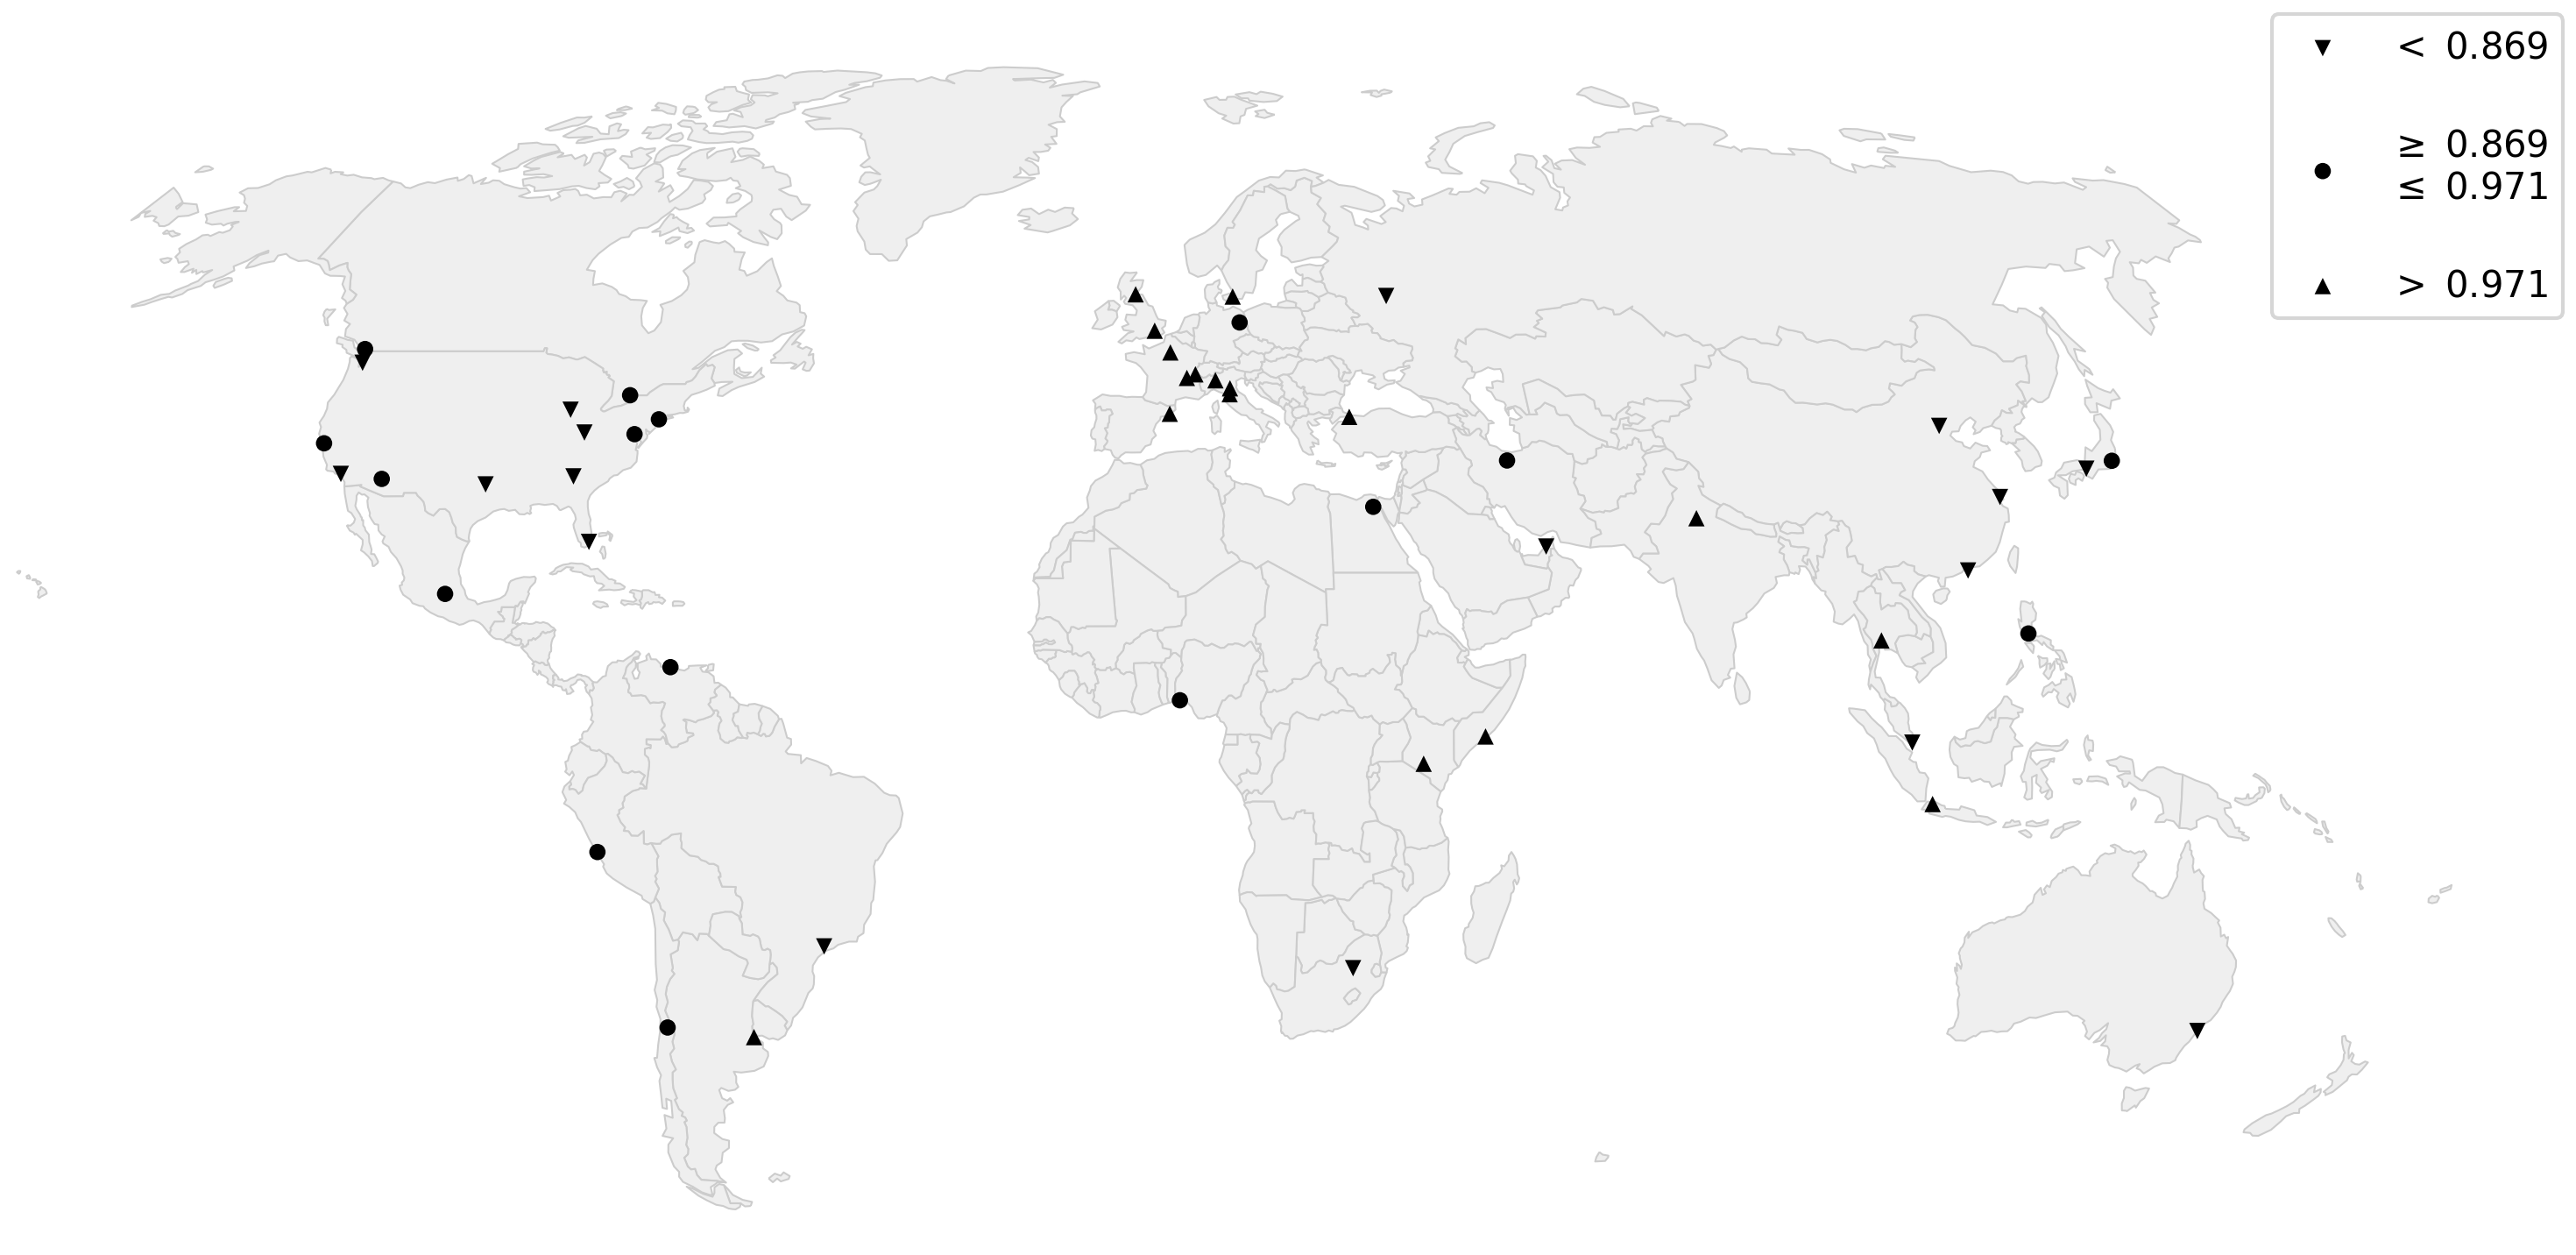
\includegraphics[width=\textwidth]{world_map_phi_bw.png}
    \caption{Map of world cities in Table \ref{tab:world_cities} grouped by SPS score tertiles.}
    \label{fig:world_map_bw}
\end{figure*}


\begin{table*}[htbp]
\centering
\caption{Indicators of nonplanarity for one square mile street networks at the centers of 50 cities worldwide. SPS = spatial planarity score = the ratio of nonplanar intersections to planar intersections. ELR = edge length ratio = the ratio of mean edge length in planar graph to mean edge length in nonplanar graph. Planar = whether street network passed a formal test of planarity.}
\label{tab:world_cities}
\begin{tabular}{ l l r r r r r r  }
\toprule
             &               & \multicolumn{3}{|c|}{Drive}         & \multicolumn{3}{c}{Walk}            \\
\midrule
Country      & City          &  Planar  &  $\phi$   &  $\lambda$   &  Planar  &  $\phi$   &  $\lambda$   \\
\midrule
Argentina & Buenos Aires &      Yes &  1.000 &  1.000 &       No &  0.946 &  0.947 \\
Australia & Sydney &       No &  0.741 &  0.749 &       No &  0.909 &  0.901 \\
Brazil & Sao Paulo &       No &  0.791 &  0.790 &       No &  0.852 &  0.831 \\
Canada & Toronto &      Yes &  0.930 &  0.958 &       No &  0.858 &  0.848 \\
          & Vancouver &       No &  0.929 &  0.948 &       No &  0.929 &  0.926 \\
Chile & Santiago &       No &  0.875 &  0.887 &       No &  0.972 &  0.971 \\
China & Beijing &       No &  0.818 &  0.872 &       No &  0.842 &  0.848 \\
          & Hong Kong &       No &  0.846 &  0.835 &       No &  0.840 &  0.818 \\
          & Shanghai &       No &  0.682 &  0.717 &       No &  0.670 &  0.659 \\
Denmark & Copenhagen &      Yes &  0.992 &  0.988 &       No &  0.991 &  0.987 \\
Egypt & Cairo &       No &  0.900 &  0.916 &       No &  0.918 &  0.906 \\
France & Lyon &       No &  0.991 &  0.989 &       No &  0.960 &  0.957 \\
          & Paris &       No &  0.988 &  0.993 &       No &  0.920 &  0.917 \\
Germany & Berlin &       No &  0.939 &  0.950 &       No &  0.943 &  0.936 \\
India & Delhi &      Yes &  1.000 &  1.000 &      Yes &  0.993 &  0.992 \\
Indonesia & Jakarta &      Yes &  0.983 &  0.986 &       No &  0.962 &  0.960 \\
Iran & Tehran &       No &  0.962 &  0.973 &       No &  0.957 &  0.956 \\
Italy & Bologna &      Yes &  1.000 &  1.000 &      Yes &  0.996 &  0.996 \\
          & Florence &      Yes &  1.000 &  1.000 &       No &  0.980 &  0.978 \\
          & Milan &      Yes &  1.000 &  1.000 &       No &  0.875 &  0.860 \\
Japan & Osaka &       No &  0.868 &  0.871 &       No &  0.951 &  0.949 \\
          & Tokyo &       No &  0.927 &  0.923 &       No &  0.922 &  0.912 \\
Kenya & Nairobi &       No &  0.974 &  0.974 &       No &  0.949 &  0.943 \\
Mexico & Mexico City &       No &  0.940 &  0.952 &       No &  0.913 &  0.917 \\
Nigeria & Lagos &       No &  0.952 &  0.967 &       No &  0.988 &  0.987 \\
Peru & Lima &       No &  0.939 &  0.941 &       No &  0.932 &  0.931 \\
Philippines & Manila &       No &  0.946 &  0.953 &       No &  0.906 &  0.895 \\
Russia & Moscow &       No &  0.574 &  0.680 &       No &  0.856 &  0.858 \\
Singapore & Singapore &       No &  0.868 &  0.874 &       No &  0.899 &  0.890 \\
Somalia & Mogadishu &      Yes &  1.000 &  1.000 &      Yes &  1.000 &  1.000 \\
South Africa & Johannesburg &       No &  0.851 &  0.883 &       No &  0.997 &  0.997 \\
Spain & Barcelona &      Yes &  1.000 &  1.000 &       No &  0.904 &  0.900 \\
Switzerland & Geneva &       No &  0.985 &  0.982 &       No &  0.828 &  0.813 \\
Thailand & Bangkok &       No &  0.988 &  0.988 &       No &  0.993 &  0.989 \\
Turkey & Istanbul &       No &  0.975 &  0.982 &       No &  0.980 &  0.978 \\
UAE & Dubai &       No &  0.685 &  0.722 &       No &  0.860 &  0.850 \\
UK & Edinburgh &       No &  0.973 &  0.968 &       No &  0.988 &  0.988 \\
          & London &       No &  0.979 &  0.981 &       No &  0.865 &  0.847 \\
USA & Atlanta &       No &  0.736 &  0.777 &       No &  0.738 &  0.724 \\
          & Chicago &       No &  0.776 &  0.814 &       No &  0.807 &  0.804 \\
          & Cincinnati &       No &  0.730 &  0.757 &       No &  0.931 &  0.927 \\
          & Dallas &       No &  0.598 &  0.650 &      Yes &  0.963 &  0.959 \\
          & Los Angeles &       No &  0.583 &  0.635 &       No &  0.793 &  0.799 \\
          & Miami &       No &  0.647 &  0.662 &       No &  0.964 &  0.961 \\
          & New York &       No &  0.881 &  0.901 &       No &  0.942 &  0.941 \\
          & Phoenix &       No &  0.955 &  0.962 &       No &  0.979 &  0.977 \\
          & San Francisco &       No &  0.935 &  0.941 &       No &  0.948 &  0.944 \\
          & Seattle &       No &  0.732 &  0.779 &       No &  0.933 &  0.926 \\
          & Washington DC &       No &  0.948 &  0.956 &       No &  0.967 &  0.967 \\
Venezuela & Caracas &       No &  0.953 &  0.957 &      Yes &  1.000 &  1.000 \\
\bottomrule
\end{tabular}
\end{table*}




\begin{figure*}[htbp]
    \center
    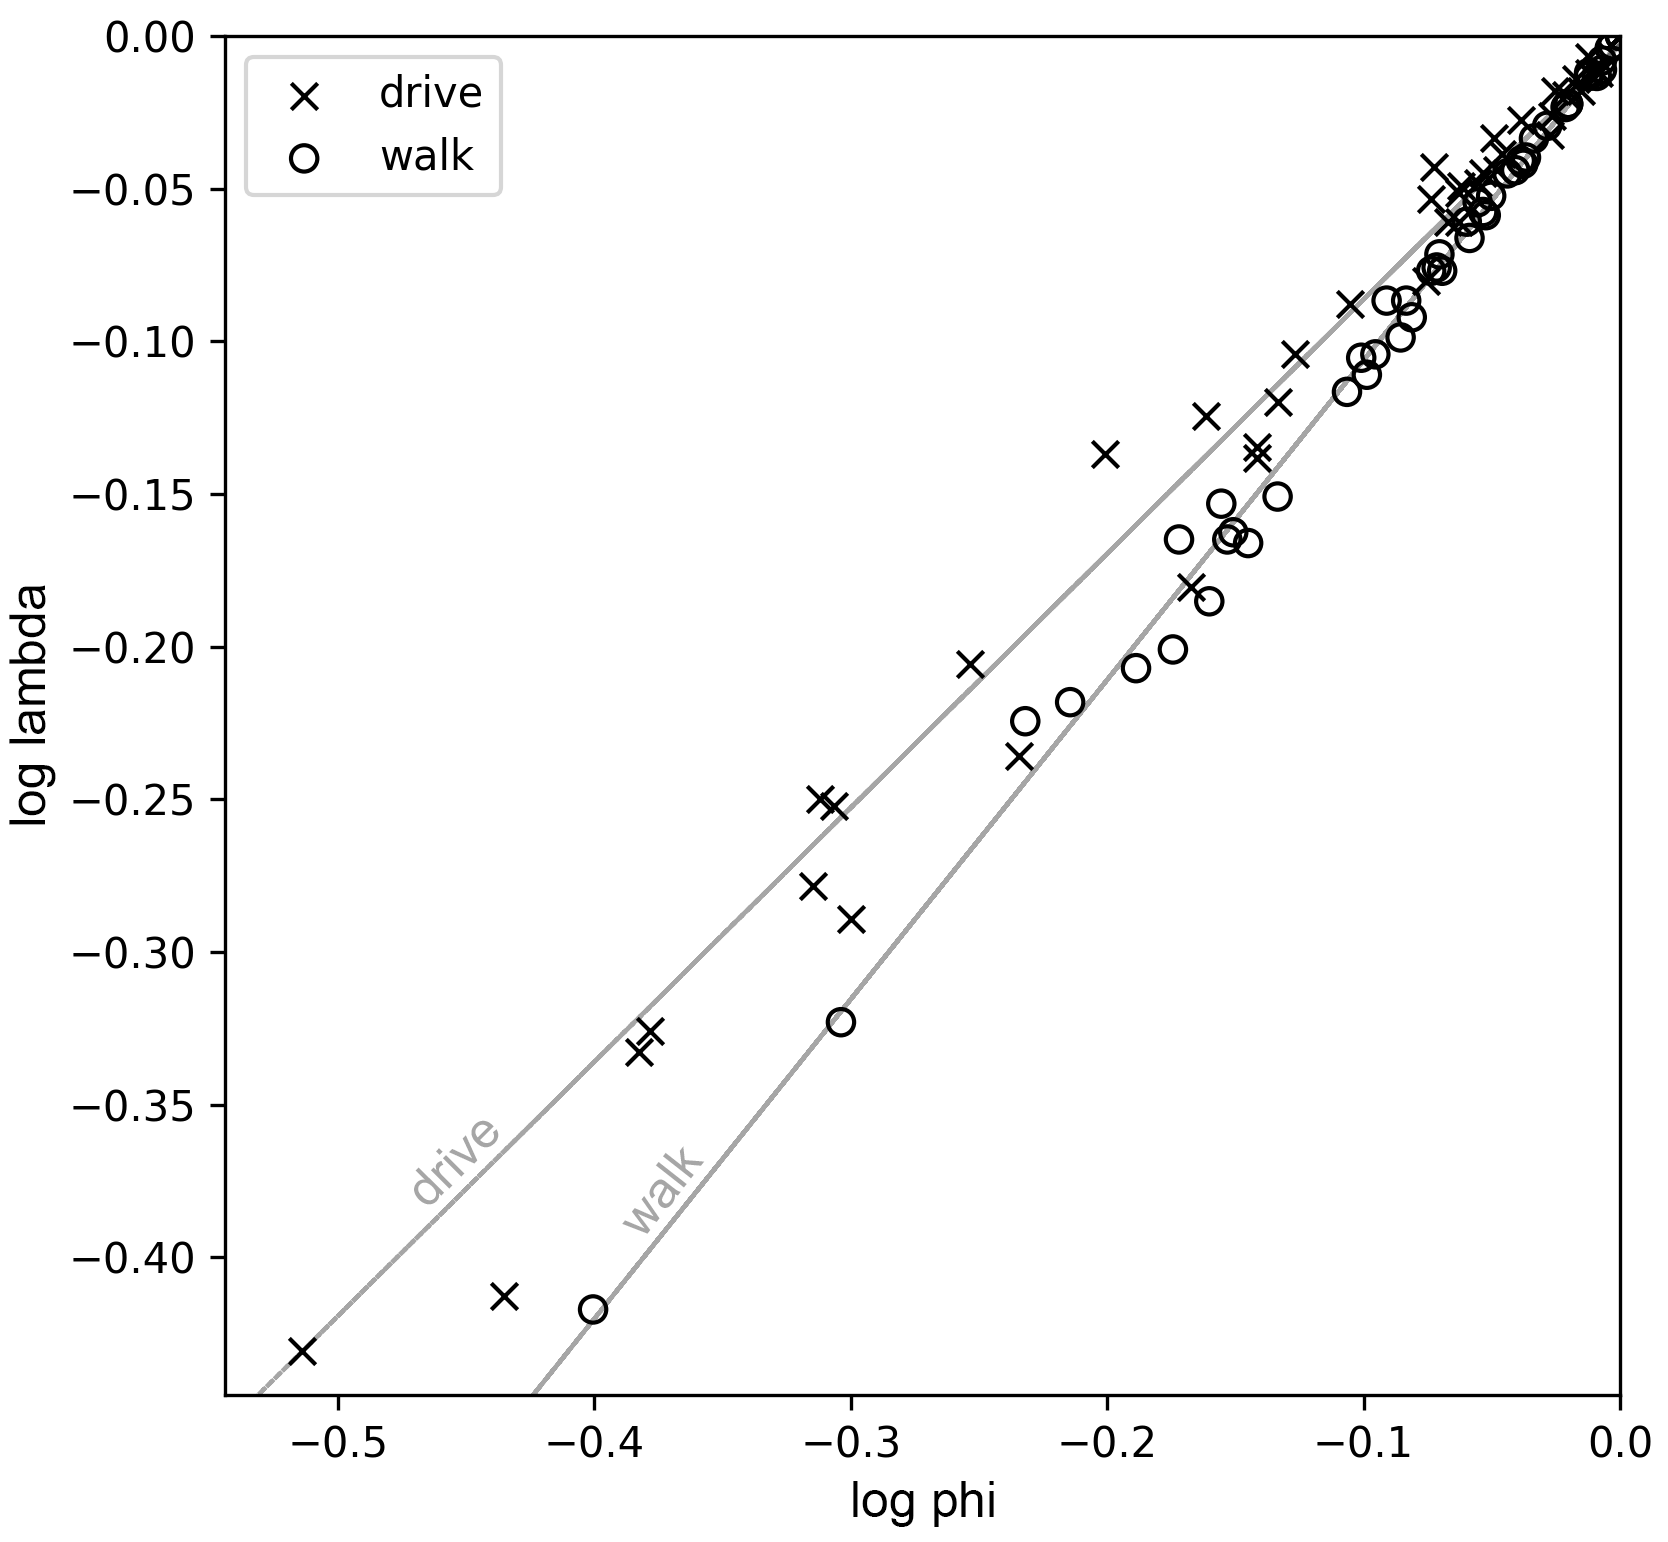
\includegraphics[width=0.5\textwidth]{regression_phi_split.png}
    \caption{Log-log plot of ELR vs SPS with simple regression lines: drive $r^2=0.98$ and walk $r^2=0.99$.}
    \label{fig:regression_split}
\end{figure*}


\subsection{A Deeper Look: Oakland, California}

We find that the street network of the entire city of Oakland is formally nonplanar when subjected to a formal mathematical test. In terms of the nonplanarity indicators, the city as a whole has a SPS score of 0.918, indicating that it is 91.8\% planar, and a ELR score of 0.936. This suggests that the planar representation of Oakland's drivable street network overstates the number of intersections (and thus, the network's connectivity) by 8.9\% city-wide (i.e., $1 / 0.918$ and understates the average edge length by 6.4\% city-wide. However, these indicators' values vary across the city.

To explore this statistical variation, we examined 100 square-mile samples of Oakland's drivable street network. Table \ref{tab:samples_city} presents descriptive statistics of these planarity indicators. 



\begin{table}[htbp]
\centering
\caption{Descriptive statistics of planarity indicators across 100 random square-mile sample runs in Oakland, California's drivable network.}
\label{tab:samples_city}
\begin{tabular}{ l r r r r }
\toprule
         &  SPR   &  ELR   \\
\midrule
count	 &    100 &   100  \\
mean     &  0.930 & 0.947  \\
$\sigma$ &  0.101 &  0.082 \\
min      &  0.569 & 0.637  \\
max      &  1.000 & 1.000  \\
\bottomrule
\end{tabular}

\end{table}






\section{Discussion}

Our findings suggest that most street networks in the centers of major cities are mathematically nonplanar but approximately planar. However, this depends on the scale of measurement: across an entire city there is likely to be some underpass or overpass somewhere, while individual neighborhoods or small suburbs might be formally planar. The type and era of urbanization is another factor. Old medieval European towns or informal settlements in the global south contain fewer grade-separated roads (and thus greater planarity) than 20th-century American or 21st-century Chinese metropolises do. This is a result of prevailing transportation technologies when the urban form was built up, as well as terrain, costs, wealth, culture, and politics.

Street networks are frequently nonplanar in the formal sense because they are spatially embedded in three dimensions --- not two --- and have a z-coordinate along with their x and y. Because they are mostly planar, typically with only a few overpasses or underpasses, they could often be described accurately as \emph{approximately planar}. However, claiming that urban street networks broadly are planar misrepresents them in several ways.

1. Forces false nodes where grade-separated edges cross.

2. Accordingly, underestimates average edge length (a proxy for street segment lengths and block sizes)

3. Misrepresents connectivity for routing, accessibility analysis, and other connectivity studies

Why are they approximately planar? Cost and politics. Expensive to build truly 3-D networks (with z-coordinates as extensive as their x- and y-coordinates) and politically infeasible.

Are street networks planar graphs? Contrary to some of the statements in the urban studies and urban physics literature, our results suggest that this cannot be universally claimed. But perhaps some of it comes down to vocabulary. If road is not synonymous with street, then a road network and a street network may not be synonymous. A road network, including freeways and boulevards, may frequently be nonplanar, but a street network, focusing on municipal streets lined by land parcels, may be at-grade and planar. But this ignores the fact that even residential streets sometimes include bridges and tunnels in hilly neighborhoods, and the fact that our analysis earlier showed that walkable circulation networks in city centers often include pedestrian tunnels and footbridges. A graph is not planar because its edges \emph{usually} or \emph{approximately} intersect only at nodes: it is planar because its edges \emph{exclusively} intersect at nodes.

Thus, street networks are not universally planar graphs. But as George Box famously stated, \enquote{All models are wrong but some are useful.} Can street networks generally be simplified to planar graphs and still be usefully well-modeled? Then answer depends on the place and on the type of analysis. In limited circumstances, where the circulation network and built form exhibit few underpasses, overpasses, or grade-separation, then perhaps yes. But universally, we must answer no.

Most egregiously, imposing planarity on a nonplanar street network forces pseudonodes at underpasses and overpasses, breaking routing and network-based accessibility modeling. For this reason, nonplanar graphs have been the standard for decades in transportation engineering, real-world traffic assignment models, and routing engines. But planar graphs are often used in the literature to study urban form and morphology. So, aside from routing, do planar graphs offer \emph{useful} models for this type of research? Again, only in limited circumstances, including examples such as the drivable networks in the three Italian cities we analyzed, which are formally planar. The results in Table \ref{tab:world_cities} show how common urban form measures such as intersection counts are overstated by planar models, while average edge lengths (a linear proxy for block size) is consequently understated. Moreover, this misrepresentation behaves inconsistently from place to place. Figure \ref{fig:world_map_bw} demonstrates how the magnitude of bias varies across cities and eras of urbanization.

So then why use planar graphs? Tractable. In some cities it doesn't matter (Italy). Polygonal analysis of urban blocks. Otherwise use nonplanar, new tools make it easy.


\section{Conclusion}

The urban studies and urban physics literatures frequently use planar graphs to urban street networks. This study demonstrated that although in limited circumstances these models may be accurate, they can behave inconsistently across different kinds of cities by misrepresenting connectivity, accessibility, routing, intersection counts and densities, and street segment lengths. It found x, y, and z. It also demonstrated how these indicators can be used to characterize the type of urbanization, in particular its three-dimensionality, of different cities. Future research can explore this latter finding, as it likely correlates with other measures of urbanization, development, and era. Finally, future research might examine how nonplanar intersection counts represent true intersections if multiple adjacent edges form multiple graph intersections at a point where only one true intersection exists from an urban design perspective.


\clearpage
\bibliographystyle{apa}
\bibliography{references}

\end{document}
